\documentclass[10pt]{article}
\usepackage[utf8]{inputenc}
\usepackage[T1]{fontenc}
\usepackage{graphicx}
\usepackage{longtable}
\usepackage{float}
\usepackage{wrapfig}
\usepackage{soul}
\usepackage{amssymb}
\usepackage{hyperref}
\parindent 0in
\usepackage[spanish]{babel}
\setlength{\parskip}{1\baselineskip}
\usepackage{fullpage}
\usepackage{multirow}
\usepackage{amsthm}
\usepackage{amsmath}
\usepackage{enumitem}
\usepackage{caption}

\newtheorem*{teorema}{Teorema}
\newtheorem*{prop}{Proposición}
\newtheorem*{lema}{Lema}

\theoremstyle{definition}
\newtheorem*{ejer}{Ejercicio}
\newtheorem*{ejem}{Ejemplo}
\newtheorem*{defi}{Definición}

\begin{document}
\begin{titlepage}
  \begin{center}

    ~\\[3cm]
    
\includegraphics[width=0.3\textwidth]{./Logo_UCM.jpg}
    ~\\[1cm]

    \textsc{\Large Asignatura: Optimización}
    
    \textsc{\small Curso 2013/2014} \\[0.5cm]
    

    \rule{0.8\linewidth}{0.5mm} \\[0.6cm]
    {\Large \bfseries Optimización de funciones de varias variables}
    \\[0.3cm] \textsc{\large Memoria de la práctica} 
    \\[0.4cm]

    \rule{0.8\linewidth}{0.5mm} \\[1.5cm]

    ~\\[3cm]
    \begin{flushright}
      {\large
      Jose Pablo Cabeza García
      
      Fracisco Criado Gallart
      }
    \end{flushright}

  \end{center}

\newpage
\mbox{}
\thispagestyle{empty}

\end{titlepage}


\setcounter{tocdepth}{3}
\tableofcontents
\newpage

\section{Introducción} \label{sec:introduccion}
En esta práctica teníamos que implementar y comparar algoritmos de optimización de $n$ variables. Hemos decidido implementar dos algoritmos sin derivadas , uno con derivadas y otro con hessiana. Además como algoritmo auxiliar para optimizar en una variable hemos implementado el algoritmo de la \textit{sección áurea}. En concreto, hemos implementado los algoritmos de \textit{Rosenbrock}, \textit{Simplex}, \textit{Steepest-Descent} y \textit{Newton-Raphson modificado}.

Para probar los algoritmos implementados hemos usado cinco funciones, tres de las cuales son estándar para problemas de optimización: \textit{Rosenbrock}, \textit{Gregory-Karney} y \textit{Rastrigin}. A añadir a éstas tres funciones, hemos desarrollado otras dos que nos parecían interesantes: la función \textit{Patata} y la función \textit{Meseta}. 

En general  mostramos los resultados de las pruebas para algunos puntos que hemos considerado representativos, junto con los parámetros del algoritmo. Además pensamos que no sólo bastaba con ver el punto inicial y final para entender por qué un algoritmo da mejores resultados o converge más rápido que otro, así que también hemos estudiado las trayectorias de los resultados de algunos de estos puntos. La relación de pruebas y algoritmos que hemos incluido en esta memoria se detalla en el \hyperref[tab:intro]{cuadro \ref*{tab:intro}}.

\begin{table}[H]\centering%
\begin{tabular}{|l|l l l l|}\cline{2-5}
\multicolumn{1}{l|}{} & \rotatebox{90}{Rosenbrock} & \rotatebox{90}{Simplex} & \rotatebox{90}{Steepest} & \rotatebox{90}{Newton-Raphson} \\ \hline
Rosenbrock            & X                          & X                       &                          &                                \\
Gregory-Kanrey        &                            &                         & X                        & X                              \\
Rastrigin             &                            & X                       &                          & X                              \\
Patata                & X                          &                         & X                        &                                \\
Meseta                &                            &                         &                          &                                \\ \hline
\end{tabular}
\caption{Relación de algoritmos-función incluidas} \label{tab:intro}
\end{table}

Todos los algoritmos los hemos implementado usando c++, con muchas funcionalidades del estándar c++ 2011. En concreto el proyecto ha sido compilado con g++ 4.7.2 con el flag ``-std=c++11'', sobre Ubuntu 12.10, usando armadillo 3.920.2 como librería para álgebra lineal y blas 1.2.2 y lapack 3.4.1 como complemento de armadillo para operaciones complejas con matrices, como la factorización de Cholesky. Para estudiar la forma de las funciones y las trayectorias de los puntos hemos usado el entorno estadístico R 3.0.2.


\section{Funciones} \label{sec:funciones}

Las funciones que hemos escogido son en su mayoría en dos dimensiones por la facilidad para estudiar de forma visual su forma y las trayectorias de las soluciones y con ello analizar mejor los algoritmos. Para probar que nuestras implementaciones funcionan para cualquier número de variables hemos añadido la función de Gregory-Karney que es de $n$ variables.

\subsection{Rosenbrock}\label{sub:fun-rosenbrock}

\begin{wrapfigure}{r}{0.5\textwidth}
  \vspace{-70pt}
  \begin{center}
    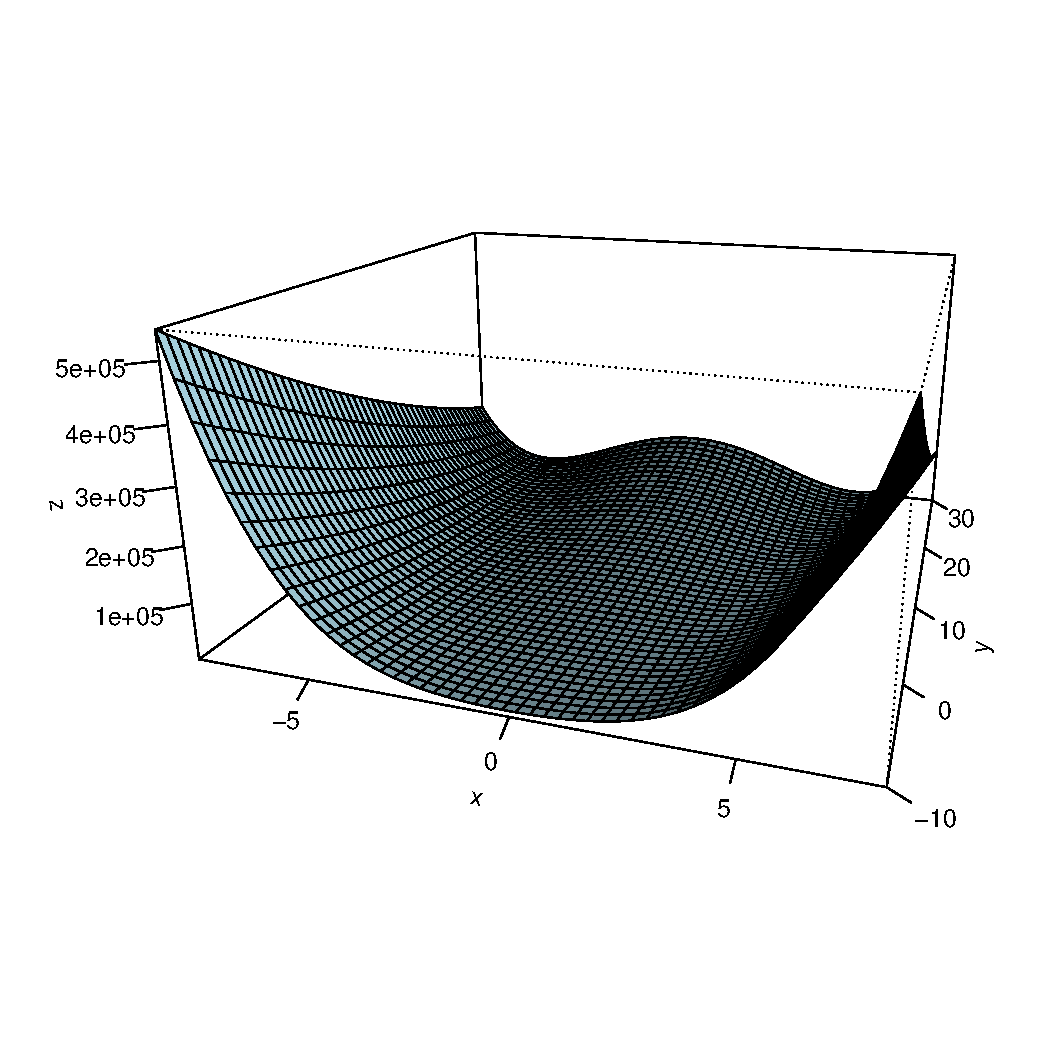
\includegraphics[width=0.48\textwidth]{../theoretic_study/func_rosenbrock/rosenbrock.pdf}
  \end{center}
  \vspace{-50pt}
  \caption{Rosenbrock}
  \vspace{-10pt}
\end{wrapfigure}

La función de Rosenbrock (conocida como funcion "banana" de
Rosenbrock) es una de las típicamente usadas para probar algoritmos de
optimización. La razón de esto es que tiene un valle ($y=x^2$). Fuera
de este valle, crece muy deprisa. Pero en el valle, tiene un mínimo
(el formado por el segundo término) con un incremento mucho menor que
el de la zona de la parábola. Así los algoritmos consiguen malos
resultados por que tienden a acercarse al valle y quedan atrapados en él.
\begin{displaymath}
Rosenbrock_a(x,y)=a(y-x^2)^2+(1-x)^2
\end{displaymath}
En la gráfica de la función casi no se nota la segunda componente.

\subsection{Gregory-Karney} \label{sub:fun-gregory-karney}

\begin{wrapfigure}{l}{0.5\textwidth}
  \vspace{-70pt}
  \begin{center}
    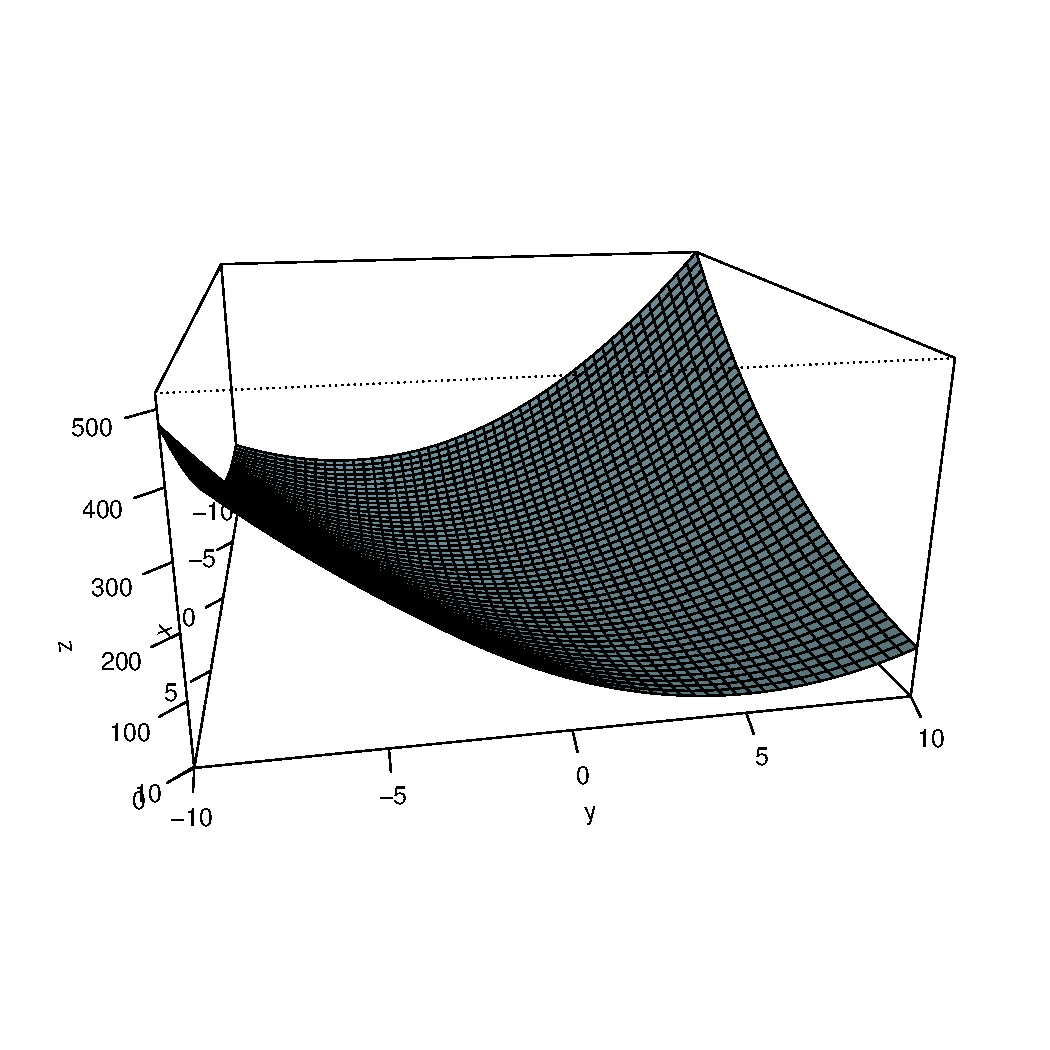
\includegraphics[width=0.48\textwidth]{../theoretic_study/func_gregory-carney/gregory.pdf}
  \end{center}
  \vspace{-60pt}
  \caption{Gregory-Karney}
  \vspace{-40pt}
\end{wrapfigure}

Hemos seleccionado la función de Gregory-Karney por ser fácil de evaluar y 
derivar (por ser casi una forma cuadrática), siendo además de varias variables.
\begin{displaymath}
	Gregory-Karney(x)=x^tAx-2x 
\end{displaymath}
\begin{displaymath}
	A=\left(\begin{array}{ccccc}
			1 & -1 & 0 & \dots & 0 \\
			-1 & 2 & -1 & \dots & 0 \\
			0 & -1 & 2 & \dots & 0 \\
			\vdots & \vdots & \vdots & \ddots & \vdots \\
			0 & 0 & 0 & \dots & 2
			\end{array}\right)
\end{displaymath}

En concreto, hemos probado 2, 3 y 5 dimensiones.

\subsection{Rastrigin} \label{sub:fun-rastrigin}

\begin{wrapfigure}{r}{0.5\textwidth}
  \vspace{-85pt}
  \begin{center}
    \includegraphics[width=0.48\textwidth]{../theoretic_study/func_rastrigin/rastrigin.pdf}
  \end{center}
  \vspace{-60pt}
  \caption{Rastrigin}
  \vspace{-50pt}
\end{wrapfigure}

La razón por la que elegimos la función de Rastrigin es para poder ver el
comportamiento de los algoritmos en funciones con varios mínimos locales. 
\begin{displaymath}
Rastrigin(x,y)=x^2+y^2-cos(18x)-cos(18y)
\end{displaymath}

El problema es que Rastrigin tiene una cantidad limitada de dichos
mínimos (motivo por el cual inventamos las dos funciones siguientes).


\subsection{Patata} \label{sub:fun-patata}

\begin{wrapfigure}{r}{0.5\textwidth}
  \vspace{-60pt}
  \begin{center}
    \includegraphics[width=0.48\textwidth]{../theoretic_study/func_patata/patata.pdf}
  \end{center}
  \vspace{-60pt}
  \caption{Patata}
  \vspace{-60pt}	
\end{wrapfigure}

Queríamos probar una función con varios mínimos locales, y decidimos
crear una propia. La funcion patata, llamada así por su parecido
localmente con una patata frita ondulada, ha sido el fruto de un
diseño en base a esos parámetros.

La definición de la función patata es como sigue:

\begin{displaymath}
	Patata(x,y)=\frac{y^2}{10} + \frac{cos((x^2+y^2)/2)}{4} - \frac{1}{x^2+y^2+1}
\end{displaymath}

Cada término tiene su razón: 
\begin{itemize}[noitemsep,nolistsep,topsep=0pt,partopsep=0pt,leftmargin=4ex,label=\textbullet]
\item El primer término garantiza que la función tienda a infinito
  lejos del origen (salvo el eje x).
\item El segundo término garantiza muchos mínimos locales, por la
  perturbación trigonométrica. 
\item El tercer término hace que el mínimo local esté en el origen sin
  que crezca demasiado para ocultar los otros mínimos locales.
\end{itemize}

\subsection{Meseta} \label{sub:fun-meseta}

% \begin{wrapfigure}{l}{0.5\textwidth}
%   \vspace{-50pt}
%   \begin{center}
%     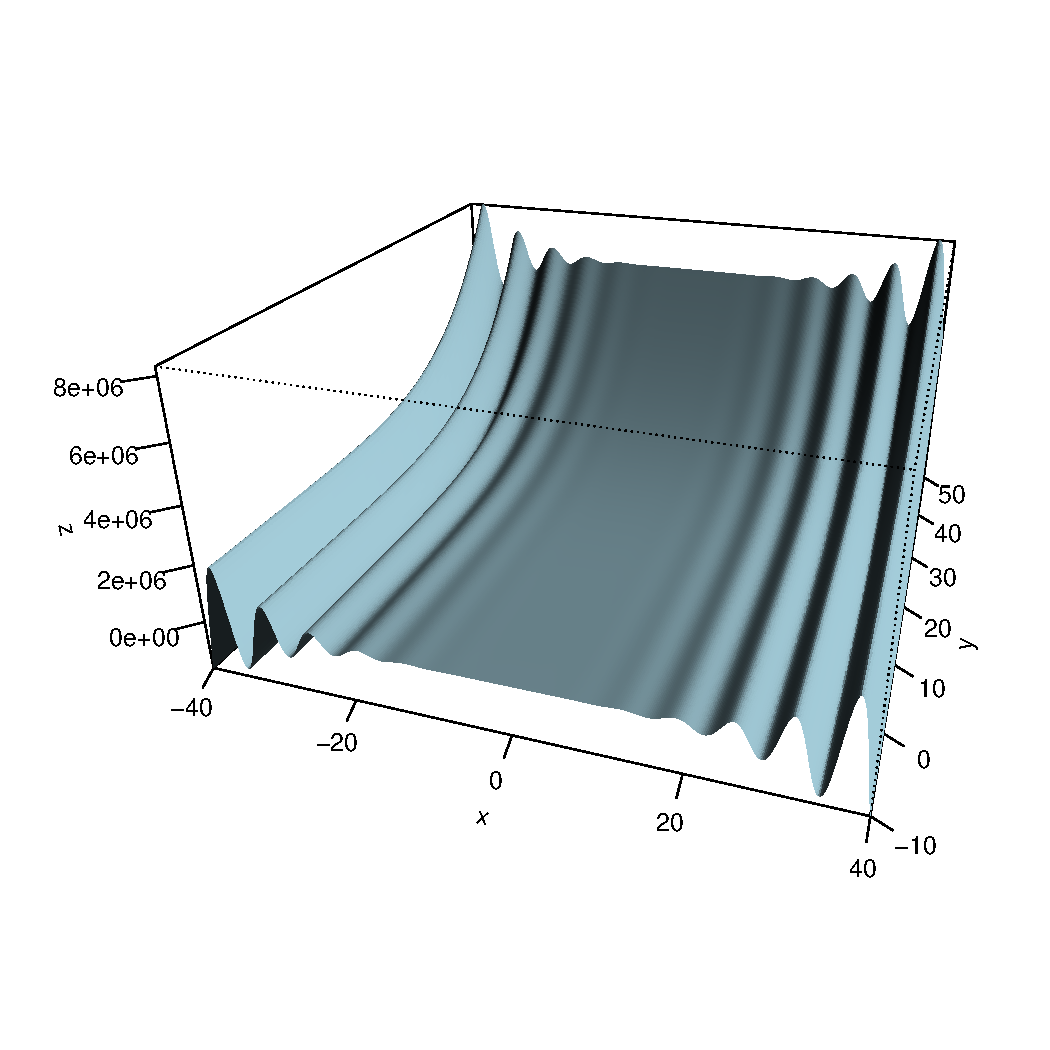
\includegraphics[width=0.48\textwidth]{../theoretic_study/func_valley/meseta.pdf}
%   \end{center}
%   \vspace{-50pt}
%   \caption{Meseta}
%   \vspace{-70pt}
% \end{wrapfigure}

La función meseta es otra función de invención propia, con los mismos principios
que la anterior. Pero se le ha dado más peso al crecimiento de los límites.
\begin{displaymath}
	Meseta(x,y)=x^4cos(x)+y^4
\end{displaymath}

De hecho, no tiene mínimo absoluto, porque el término coseno puede ser
arbitrariamente pequeño. Por esto, queríamos comprobar en qué mínimo
se quedan los algoritmos, ya que el término coseno actúa como niveles
barrera.

\begin{figure}[H]\centering%
  \vspace{-3em}%
  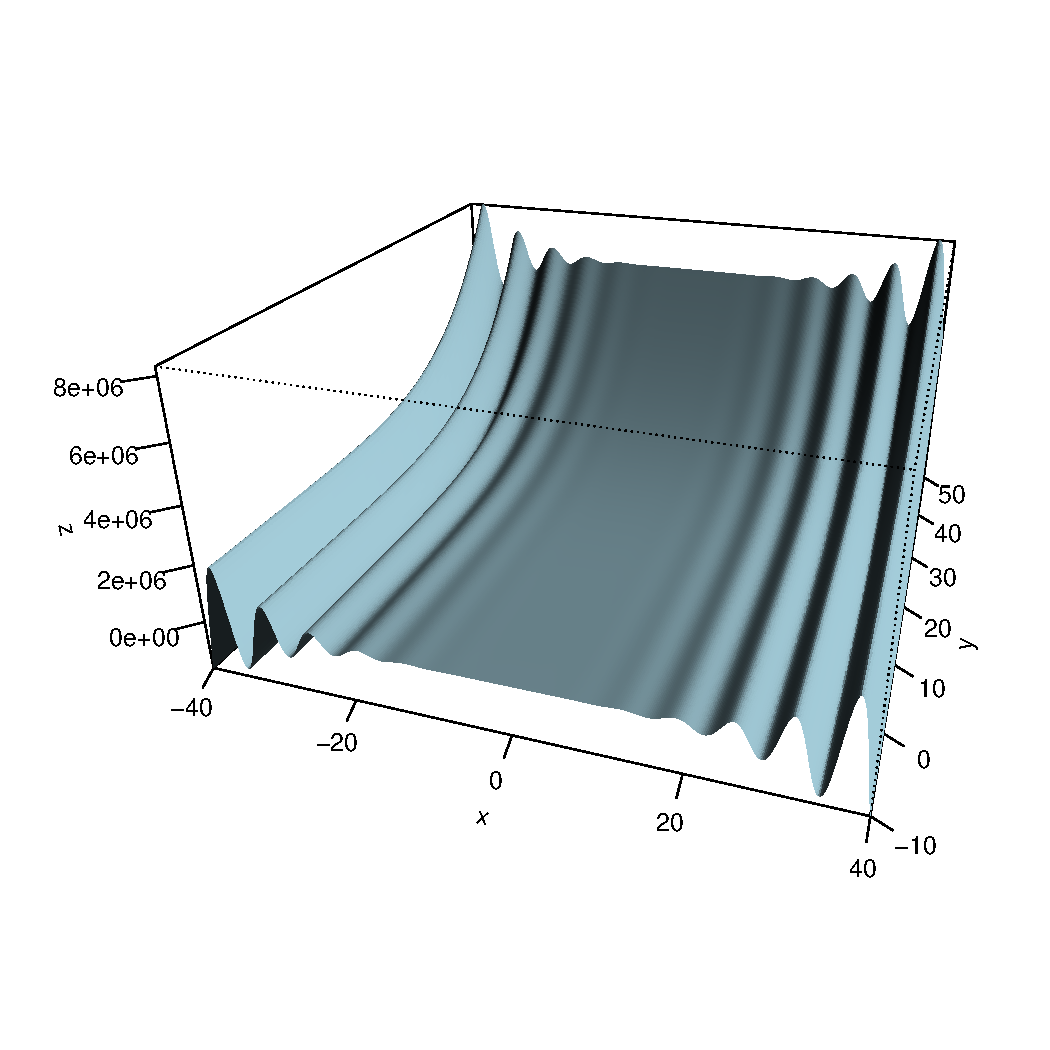
\includegraphics[width=0.5\textwidth]{../theoretic_study/func_valley/meseta.pdf}
  \vspace{-3em}%
  \caption{Meseta}
\end{figure}



\section{Algoritmos}
Aquí hemos analizado un poco los algoritmos que hemos implementado, añadiendo algunos resultados significativos de cómo han funcionado. Sobre los estudios de las trayectorias de las soluciones, decir que el punto negro es el inicial y el blanco el final, indicando el color de los puntos intermedios el ``sentido'' de la trayectoria, siendo rojo el inicial y amarillo el final.

\subsection{Rosenbrock} \label{sub:alg-rosenbrock}

El algoritmo de rosenbrock se basa en el proceso de ortonormalización de Gram-Schmidt para generar una base ortonormal. Tras esto, se optimiza en dichas direcciones, generando una series de puntos que después se usaran para construir otra base ortonormal y repetir el proceso.

Entre los problemas que se nos plantearon con el alg. lineal estaba el del punto iniciale y el $\epsilon$ a usar. Para resolver el primero tomamos el punto a partir del cual restringíamos con un tamaño de paso (de 1000 a 100000). Para el problema del $\epsilon$ de parada, sencillamente pasamos el que usamos en el algoritmo. El criterio estándar seguido es: $|| f(x_k) - f(x_{k+1}) || < \epsilon$  o $|| f(x_{k+1} ||< \epsilon$
% \begin{displaymath}
%   \begin{array}{l@{ \hspace{3ex}\textrm{ o }\hspace{3ex} }r} 
%     || f(x_k) - f(x_{k+1}) || < \epsilon & || f(x_{k+1} < \epsilon || \\ \end{array}
% \end{displaymath}


Estos son algunos resultado usando el algoritmo de la sección áurea como algoritmo de optimización lineal:
\begin{table}[H]
\hfill\begin{tabular}{|c|cccccc|c|} \hline
\bf point  & \bf eps & \bf maxit & \bf path & \bf eval & \bf diff    & \bf final           & \bf function                \\\hline\hline
(0,0)      & 0.0005  & 10000     & 10000    & 1360002  & -81.1848    & (-8.06544,65.0564)  & \multirow{4}{*}{Rosenbrock} \\
(10,-10)   & 0.0005  & 10000     & 10000    & 1360002  & 1.20956e+06 & (-21.7229,471.89)   &                             \\
(0,10)     & 0.0005  & 10000     & 10000    & 1360002  & 9272.37     & (27.9931,783.614)   &                             \\
(-1,1)     & 0.0005  & 10000     & 2        & 274      & 4           & (0.999968,0.99994)  &                             \\\hline\hline
(0.001,10) & 0.0005  & 10000     & 7        & 954      & 10.2313     & (-122.76,-0.71873)  & \multirow{3}{*}{Patata}     \\
(10,10)    & 0.0005  & 10000     & 10000    & 1360002  & 10.2107     & (833.428,-0.85336)  &                             \\
(10,0)     & 0.0005  & 10000     & 10000    & 1360002  & 0.23134     & (49.5971,0.0256535) &                             \\\hline
\end{tabular}\hfill\hbox{}
\caption{Resultados del algoritmo de Rosenbrock}
\end{table}
\vspace{-1em}

\begin{wrapfigure}{r}{0.6\textwidth}
\vspace{-8.6em}\hfill%
\hspace{-6ex}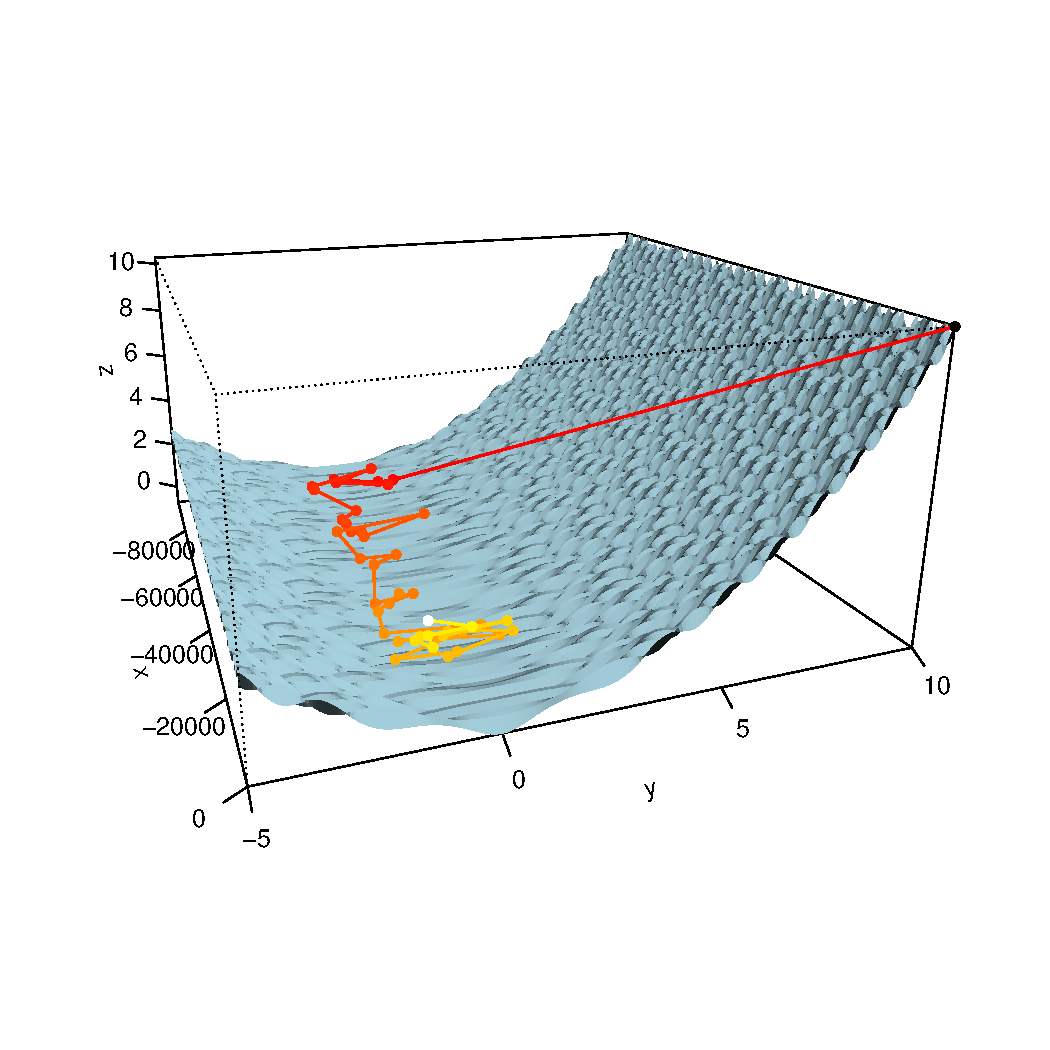
\includegraphics[width=1.2\linewidth]{../theoretic_study/func_patata/R/0,10/plot3.pdf}%
\hfill\hbox{}
\vspace{-8em}
\caption{\small función patata y sec. aurea con paso de 100000, $x_0=(0,10)$} \label{fig:rosen1}
\vspace{-5em}
\end{wrapfigure}
Como se puede ver por los resultados, a pesar que el algoritmo comience en un punto relativamente cercano a un mínimo global, tiende a alejarse considerablemente de éste, siendo la mayoría de los puntos finales alejados del origen. La \hyperref[fig:rosen1]{Figura \ref*{fig:rosen1}} en la que el algoritmo se aleja del mínimo global $(0,0)$ en la primera iteración, es un ejemplo claro de esto.

La razón de esto es que el algoritmo carece de información del entorno del punto, tan solo conoce la información obtenida al mejorar iterativamente por las rectas, dando casos muy malos como el del primer punto, en el cual se llega incluso a empeorar. 
\newpage
% Esto podría deberse al algoritmo de optimización lineal que hemos implementado, pero por lo general la tendencia se debería mantener independientemente del algoritmo que se use.

\begin{wrapfigure}{l}{0.5\textwidth}
\vspace{-4em}\hfill%
\hspace{-5ex}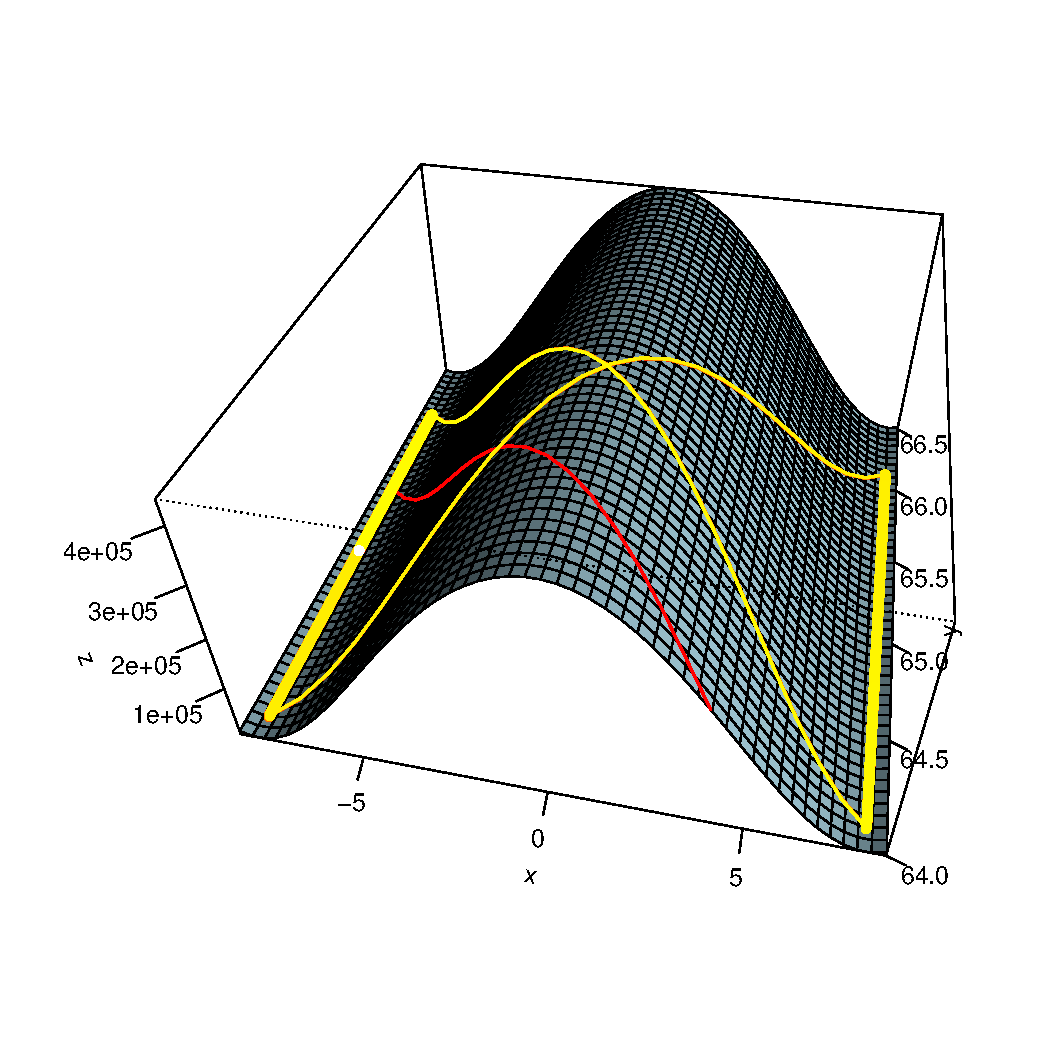
\includegraphics[width=1\linewidth]{../graphs/rosenbrock_fun/rosen/rosen_plot3.pdf}%
\hfill\hbox{}
\vspace{-4em}
\caption{\small ciclos en la función de rosenbrock con $x_0=(0,0)$} \label{fig:rosen2}
\vspace{-4.5em}
\end{wrapfigure}

Otro caso que cabe destacar es el reflejado en la \hyperref[fig:rosen2]{Figura \ref*{fig:rosen2}}. En este caso concreto el algoritmo salta de un lado al otro del valle tras unos cientos de iteraciones, terminando cuando ha agotado su número máximo de iteraciones.

Este caso es recurrente. Los puntos que se van obteniendo están contenidos en unos ciertos intervalos que se repiten tras algunas iteraciones. Esto puede ser debido a la manera en la que se genera una nueva base a partir de la anterior por el método de Gram-Schmidt, que no es capaz de generar la sufiente ``diversidad'' de bases y éstas terminan repitiendose, generando ciclos en las soluciones.


\subsection{Simplex} \label{sub:alg-simplex}
\begin{wrapfigure}{r}{0.4\linewidth}
\vspace{-6.5em}\centering%
\hspace{-4ex}%
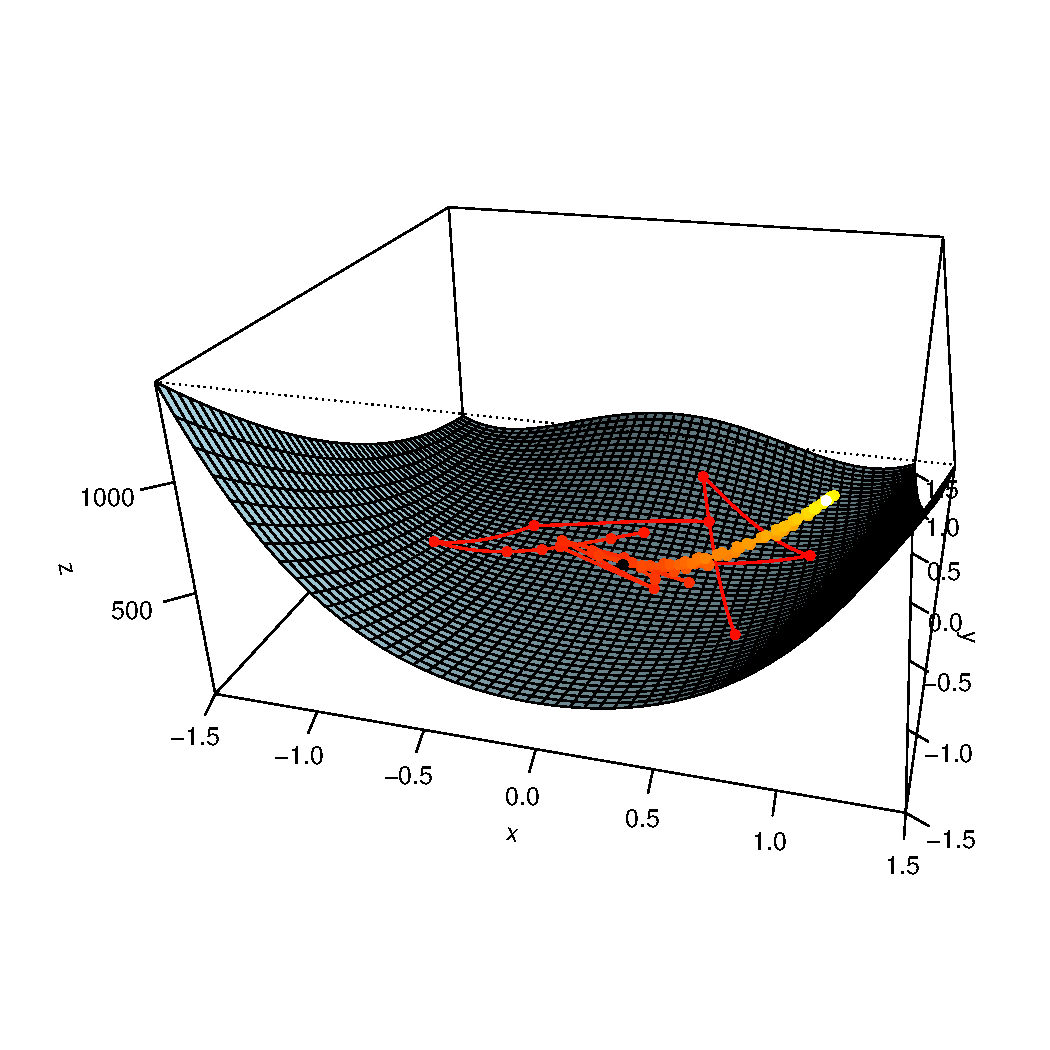
\includegraphics[width=1.1\linewidth]{../graphs/rosenbrock_fun/simplex/plot1.pdf}%
%\hfill\hbox{}
\vspace{-5em}
\caption{\small función rosenbrock  con $x_0=(0,10)$} \label{fig:rosen1}
%\vspace{-5em}
\end{wrapfigure}
Hemos implementado el algoritmo de Simplex de Nelder-Mead. Éste
algoritmo mantiene un simplex de $n+1$ que va modificando para
aproximarse a mínimos. En la implementación, el algoritmo usa una
serie de parámetros que hemos puesto defecto como: $\alpha=0.5$,
$\beta=2.0$, $\gamma=0.5$, $\delta=0.5$ y $s=1.0$.

La ventaja de este algoritmo frente al resto de los que hemos
implementado es que no hace uso de algoritmos auxiliares que puedan
complicar el análisis del algoritmo. Además la información que tiene
del en tormo por el simplex hace que pueda ``esquivar'' situaciones de
riesgo para otros algoritmos.

\begin{table}[H]\centering%
\begin{tabular}{|l|lllll|l|} \hline
\bf point                           & \bf  path & \bf  eval & \bf  diff   & \bf  final                & \bf  value  & \bf  function               \\ \hline\hline
(0,0)                               & 92        & 93        & 0.999836    & (0.993342,0.985634)       & 0.000164134 & \multirow{4}{*}{rosenbrock} \\
(10,-10)                            & 132       & 133       & 1.21008e+06 & (0.994107,0.987556)       & 8.27962e-05 &                             \\
(0,10)                              & 125       & 126       & 10001       & (1.00989,1.02081)         & 0.000184334 &                             \\
(-1,1)                              & 135       & 136       & 3.99974     & (1.01168,1.02239)         & 0.000258348 &                             \\ \hline\hline
(2,2)                               & 54        & 55        & 10.2547     & (-0.00267934,0.000804213) & -1.99872    & \multirow{4}{*}{rastrigin}  \\
($\frac{\pi}{6}$, $\frac{\pi}{6}$)  & 46        & 47        & 0.00107796  & (0.346058,0.345578)       & -1.75738    &                             \\
($\frac{\pi}{3}$, $\frac{2\pi}{9}$) & 44        & 45        & 0.614837    & (0.694339,0.695292)       & -1.03083    &                             \\
(6,6)                               & 67        & 68        & 72.1587     & (-1.03931,0.000519967)    & -0.90973    &                             \\ \hline
\end{tabular}%
\caption{Resultados del algoritmo del simplex con $epsilon=0.0005$}%
\end{table}
\vspace{-1.5em}


\hfill\begin{minipage}{\textwidth}
\hspace{-3ex}\begin{wrapfigure}{l}{0.4\linewidth}
\vspace{-4.5em}
\includegraphics[width=0.9\linewidth]{../graphs/rastrigin_func/simplex/plot1.pdf}%
\vspace{-3.5em}
\caption{\small función de rastrigin con $x_0=(0,10)$}
\vspace{-5em}
\end{wrapfigure}
Como puede verse por las figuras, la trayectoria de los puntos que
evalúa el algoritmo en dos de los casos de prueba al principio están
casi sin patrón, pero en seguida se convergen en a la dirección
correcta.

\vspace{\baselineskip}
Cabe destacar que de todos, es el único algoritmo en el que no hemos
encontrado ningún caso demasiado malo. Además el número de
evaluaciones que hace de la función es mínima en comparación con los
otros.%
\end{minipage}\hfill\hbox{}

\vspace{-4em}
\subsection{Steepest Descent} \label{sub:alg-steepest}

El algoritmo de steepest-descent hace uso del gradiente de la función a optimizar para buscar la dirección de máximo descenso que es tangente al punto dado. Entonces el algoritmo optimiza en dicha dirección de descenso usando un algoritmo auxiliar de optimización lineal. A parte del criterio de parada estándar también se usa el criterio $|| - \bigtriangledown f(x_k) || < \epsilon $

\begin{wrapfigure}{r}{0.5\textwidth}
\vspace{-4.8em}%
\hfill%
\hspace{-6ex}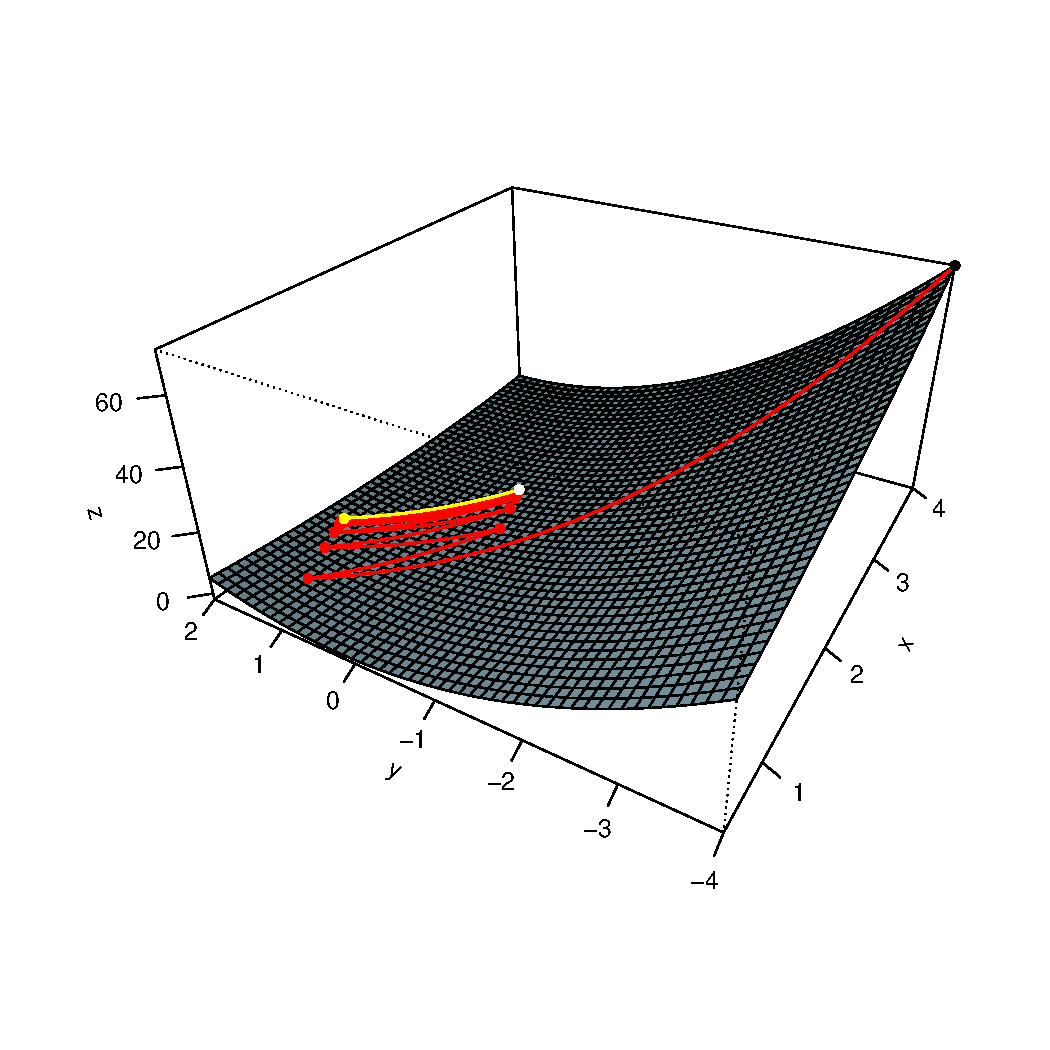
\includegraphics[width=0.9\linewidth]{../graphs/gregory_fun/steep/steep.pdf}%
\hfill\hbox{}
\vspace{-3.5em}
\caption{\small gregory-karney en $x_0=(4,-4)$ del \hyperref[tab:steep]{cuadro \ref*{tab:steep}}} \label{fig:steep1}
\vspace{-3em}
\end{wrapfigure}

Para implementarlo usamos el algoritmo de la sección áurea para optimizar en las rectas, con el mismo criterio que en el algoritmo de \hyperref[sub:alg-rose]{rosenbrock}. Este algoritmo en general da buenos resultados, aproximándose a mínimos locales de forma efectiva. 

Uno de los problemas que tenemos con nuestra implementación es el ``underflow'' y ``overflow'' cuando tiende el resultado a 0 o a infinito. Concretamente los NaN de la tabla inferior se deben a que al evaluar el punto final en la función resulta en un valor que excede la capacidad del tipo básico de la máquina, resultando en un valor infinito en uno de los pasos intermedios de la evaluación de la función.

Aquí un cuadro con los resultados de algunas de las pruebas que hemos realizado:

\begin{table}[H]
\hfill\begin{tabular}{|c|cccccc|c|}\hline
\bf point   & \bf path & \bf eval & \bf grad & \bf diff        & \bf final                         & \bf value ($\approx$) & \bf function                    \\\hline\hline
(0.001,10)  & 1001     & 67002    & 1001     & 10.2313         & (8.97279e-71,-1.40843)            & -2.4e-06              & \multirow{3}{*}{patata}         \\
(10,10)     & 503      & 33636    & 503      & -nan            & (4.87463e+154,443.202)            & -nan                  &                                 \\
(10,0)      & 76       & 5027     & 76       & -nan            & $\approx$(1.34e+156,0)            & -nan                  &                                 \\\hline\hline
(4,4)       & 1001     & 67002    & 1001     & 8.00037         & $\approx$(1.54,1.74)              & -0.0004               & \multirow{7}{*}{gregory-karney} \\
(-4,-4)     & 1001     & 67002    & 1001     & 23.9994         & (2.45958,0.25639)                 & 0.0006                &                                 \\
(4,-4)      & 1001     & 67002    & 1001     & 72.0007         & (2.45942,0.256639)                & -0.0007               &                                 \\
(0,0,0)     & 1001     & 67002    & 1001     & $\approx$0.0007 & $\approx$(2.68,2.71,0.43)         & -0.0007               &                                 \\
(3,3,3)     & 1001     & 67002    & 1001     & 2.99967         & $\approx$(3.32,1.29,1.57)         & 0.0003                &                                 \\
(0,0,0,0,0) & 1001     & 67002    & 1001     & $\approx$0.003  & $\approx$(4.8,4.53,2.3,2.63,0.62) & -0.003                &                                 \\
(5,5,5,5,5) & 1001     & 67002    & 1001     & 14.9957         & $\approx$(5.2,3.47,3.7,1.36,1.3)  & 0.004                 &                                 \\\hline
\end{tabular}\hfill\hbox{}
\caption{Resultados del algoritmo de steepest-descent con $\epsilon=0.0005$} \label{tab:steep}
\end{table}
\vspace{-1em}

\begin{wrapfigure}{l}{0.5\textwidth}
\vspace{-5.3em}%
\hfill%
\hspace{-6ex}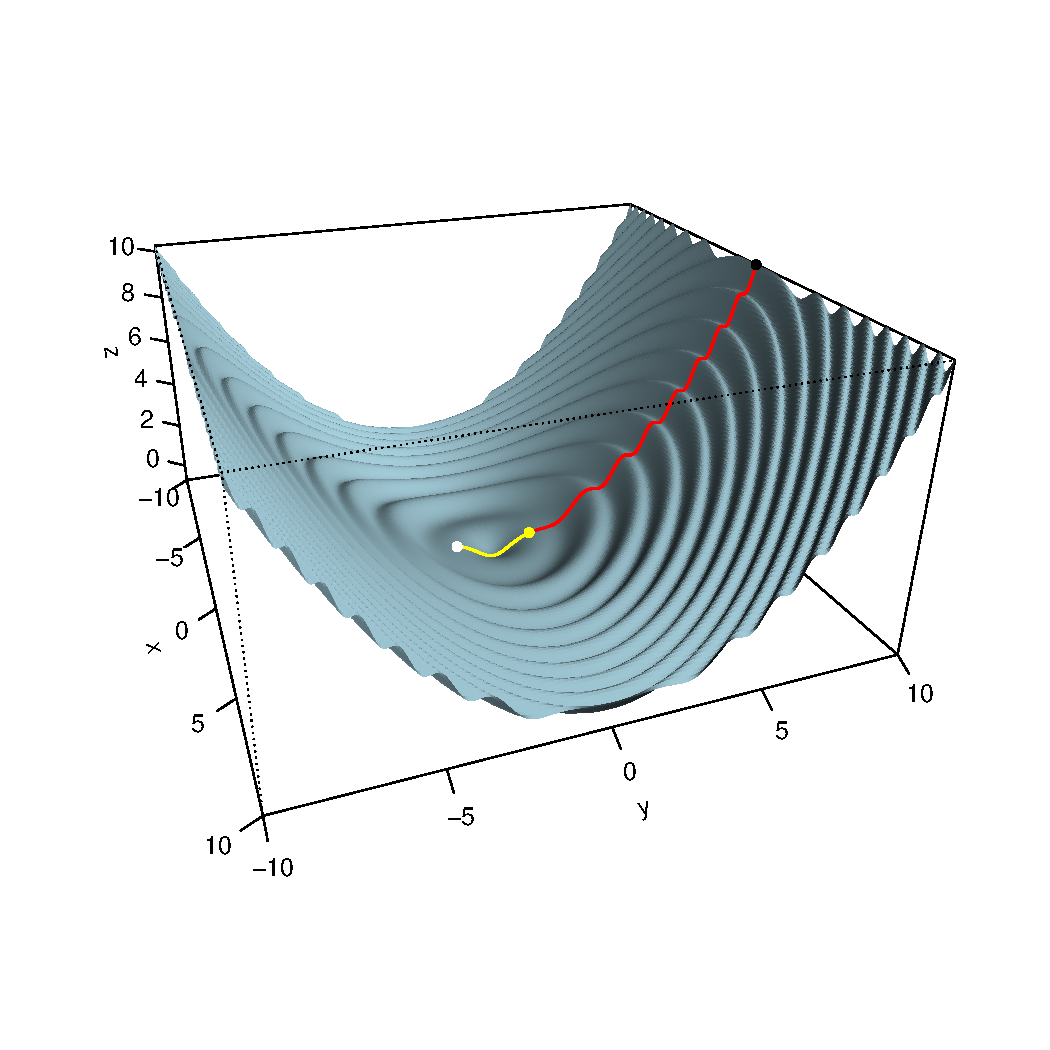
\includegraphics[width=0.9\linewidth]{../graphs/patata_func/steep/steep.pdf}
\hfill\hbox{}
\vspace{-3.5em}
\caption{\small f. patata en $x_0=(0.001,10)$ del \hyperref[tab:steep]{cuadro \ref*{tab:steep}}} \label{fig:steep2}
\vspace{-4.5em}
\end{wrapfigure}


Hay que señalar que al igual que con el algoritmo de \hyperref[sub:alg-rosen]{rosenbrock}, se pueden producir ciclos que hagan que a partir de cierto punto no se mejore más la solución conseguida.

Un caso de esto es la figura del latera, que muestra comoel algoritmo comienza a saltar entre puntos con pendiente muy plana, hasta llegar al máximo de iteraciones programado. Esta figura es ilustrativa ya que si se compara con la \hyperref[fig:rosen1]{figura \ref*{fig:rosen1}} del algoritmo de rosenbrock, steepest-descent es capaz de encontrar la dirección correcta en la que optimizar.

\subsection{Newton-Raphson (Con factorización de Cholesky)} \label{sub:alg-newton-raphson}

El algoritmo de Newton-Raphson modificado utiliza la idea básica de los 
algoritmos de Newton pero utilizando la factorización de Cholesky para 
resolver el sistema lineal (porque la hessiana es simétrica).

\begin{wrapfigure}{l}{0.5\linewidth}
\vspace{-4em}%
\hfill%
\hspace{-6ex}\includegraphics[width=0.9\linewidth]{../graphs/rastrigin_func/newt_0.34/plot1.pdf}
\hfill\hbox{}
\vspace{-3.5em}
\caption{\small f. rastrigin en $\frac{\pi}{6}$, $\frac{\pi}{6}$ del \hyperref[tab:newt]{cuadro \ref*{tab:newt}}} \label{fig:steep2}
\vspace{-5.5em}
\end{wrapfigure}

En esta parte hemos hecho uso de la factorización de Cholesky de armadillo para factorizar la hessiana y resolver el sistema con el gradiente. Esto tenía el problemas de que en ciertos casos que no hemos incluido aquí, la factorización no convergía.


En general ha dado buenos resultados para los casos que hemos probado en los que convergía, incluso hemos incluido pruebas para Gregory-Karney con 3 y 5 dimensiones. A pesar de sus buenos resultados puede observarse en las figuras que nuevamente se producen ciclos en el algoritmo.
\vspace{2.8em}

\begin{table}[H]
\hfill\begin{tabular}{|c|ccccccc|c|} \hline
\bf point                           & \bf path & \bf eval & \bf grad & \bf hess & \bf diff($\approx$) & \bf final                    & \bf value ($\approx$) & \bf function               \\\hline\hline
(4,4)                               & 1001     & 69002    & 1001     & 1001     & 7.99                & (1.10557,-0.341646)          & 1.43e-05              & \multirow{8}{*}{G-K}       \\
(-4,-4)                             & 1001     & 69002    & 1001     & 1001     & 24                  & (3.66405,2.3867)             & -0.0001               &                            \\
(4,-4)                              & 1001     & 69002    & 1001     & 1001     & 72                  & (2.32879,0.178013)           & -3.7e-05              &                            \\
(0,0,0)                             & 1001     & 69002    & 1001     & 1001     & 0.0002              & * & -0.0002               &                            \\
(3,3,3)                             & 1001     & 69002    & 1001     & 1001     & 2.99                & (3,2.70714,2.41428)          & 0.0003                &                            \\
(0,0,0,0,0)                         & 1001     & 69002    & 1001     & 1001     & 0.0003              & **                            & -0.00037              &                            \\
(5,5,5,5,5)                         & 1001     & 69002    & 1001     & 1001     & 14.99               & (5,4.5,4,3.5,3)              & 0.0003                &                            \\ \hline\hline
(2,2)                               & 21       & 1382     & 21       & 21       & 8.07                & (1.04076,1.04076)            & 0.179                 & \multirow{4}{*}{rastrigin} \\
($\frac{\pi}{6}$, $\frac{\pi}{6}$)  & 8        & 485      & 8        & 8        & -1.93               & (1.04076,1.04076)            & 0.179                 &                            \\
($\frac{\pi}{3}$, $\frac{2\pi}{9}$) & 1001     & 69002    & 1001     & 1001     & -0.42               & (0.118408,0.0550001)         & 5.812e-07             &                            \\
(6,6)                               & 17       & 1106     & 17       & 17       & 71.07               & (1.04076,1.04076)            & 0.179                 &                            \\ \hline
\end{tabular}\hfill\hbox{}

\vspace{1ex}{\hspace{1ex} \scriptsize * (1.1e-4,7.357e-05,3.678e-05) \hspace{2ex}** (1.9e-4,1.5e-4,1.1e-4,7.3e-05,3.6e-05)}
\caption{Resultados de newton-raphson con $epsilon=0.0005$}\label{tab:newt}
\end{table}
\vspace{-4em}
\begin{table}[H]\centering
\begin{tabular}{cc}
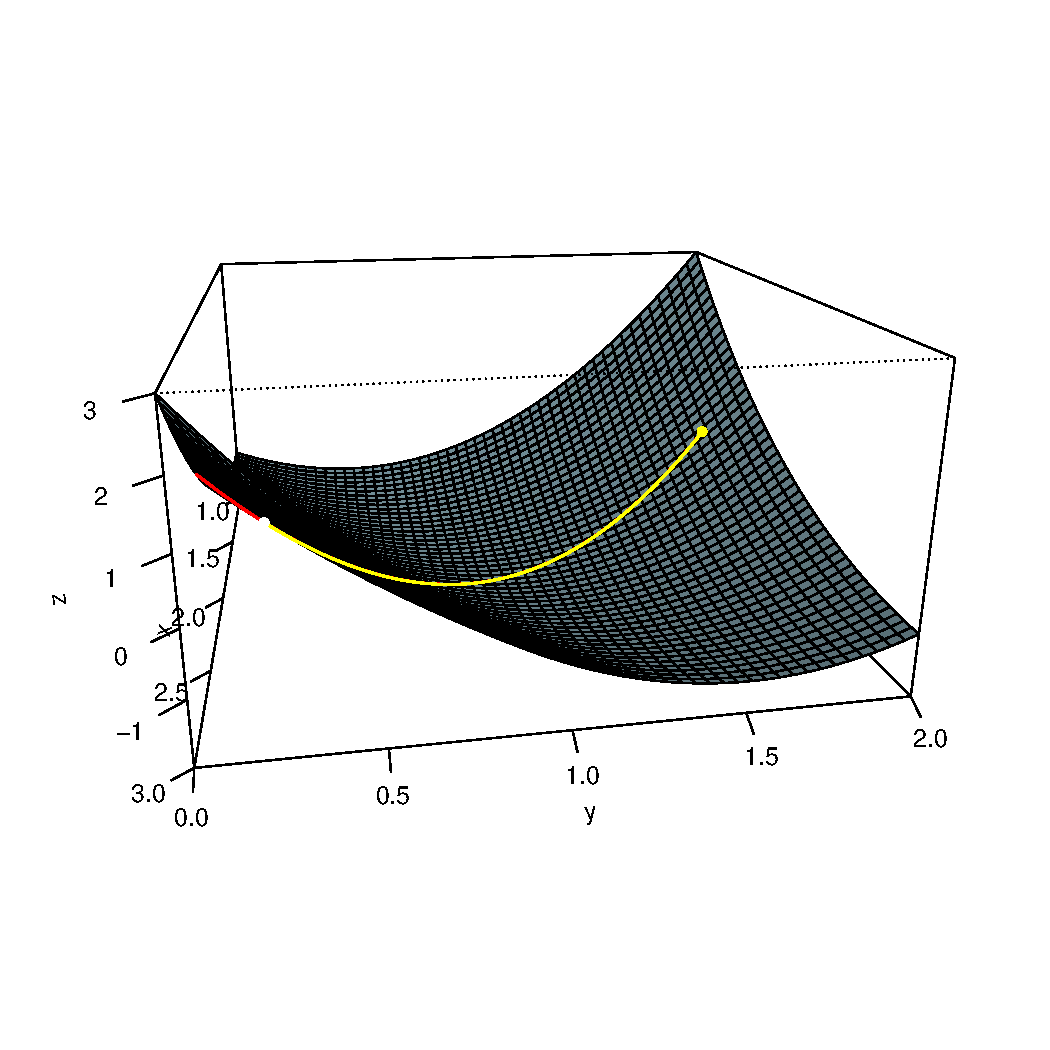
\includegraphics[width=0.4\linewidth]{../graphs/gregory_fun/newt/newt1.pdf}
&
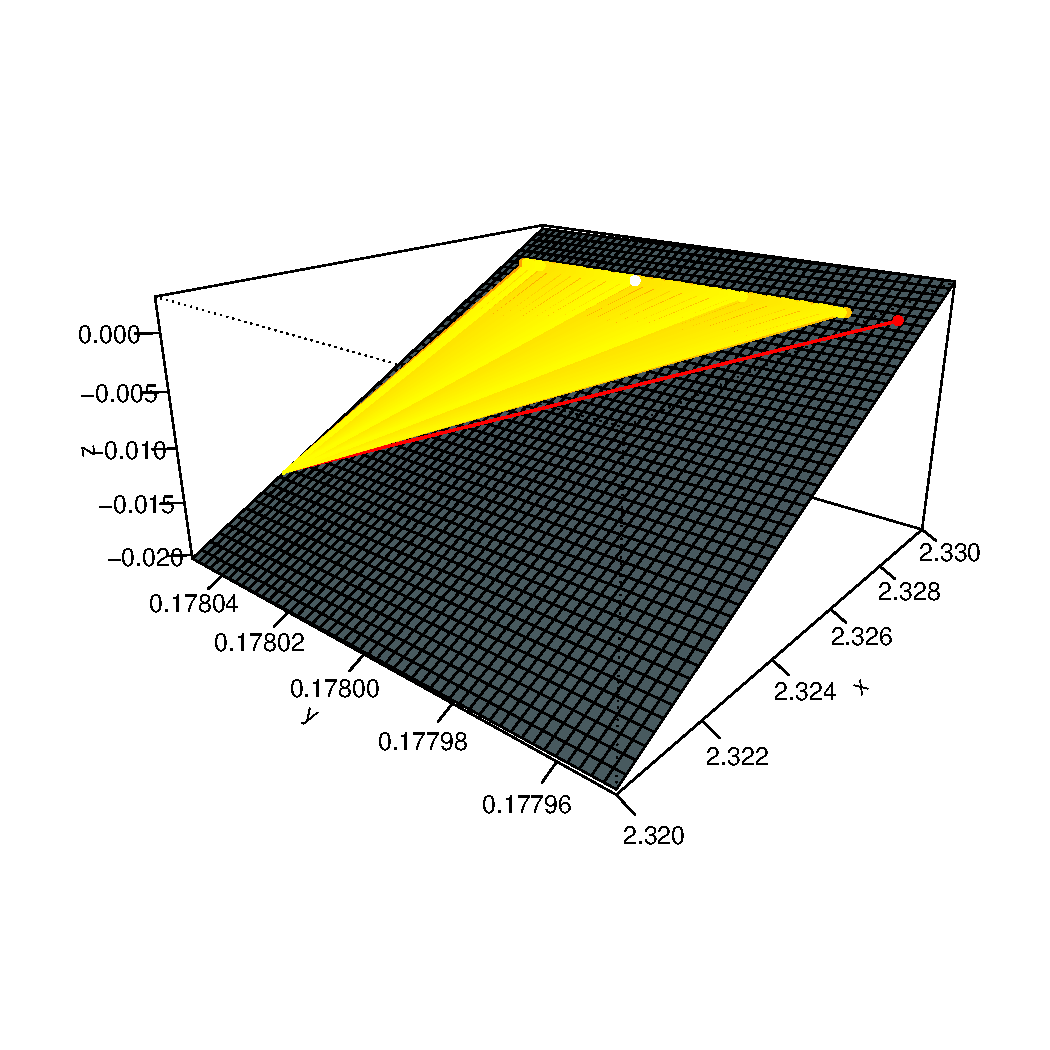
\includegraphics[width=0.4\linewidth]{../graphs/gregory_fun/newt/newt2.pdf}\\[-3em]
Figura. {\small función G-K en $x_0=(4,-4)$}&
Figura. {\small detalles de función G-K en $x_0=(4,-4)$}\\
\end{tabular}
\end{table}

% \begin{tabular}{c@{\hfill}c}\
% 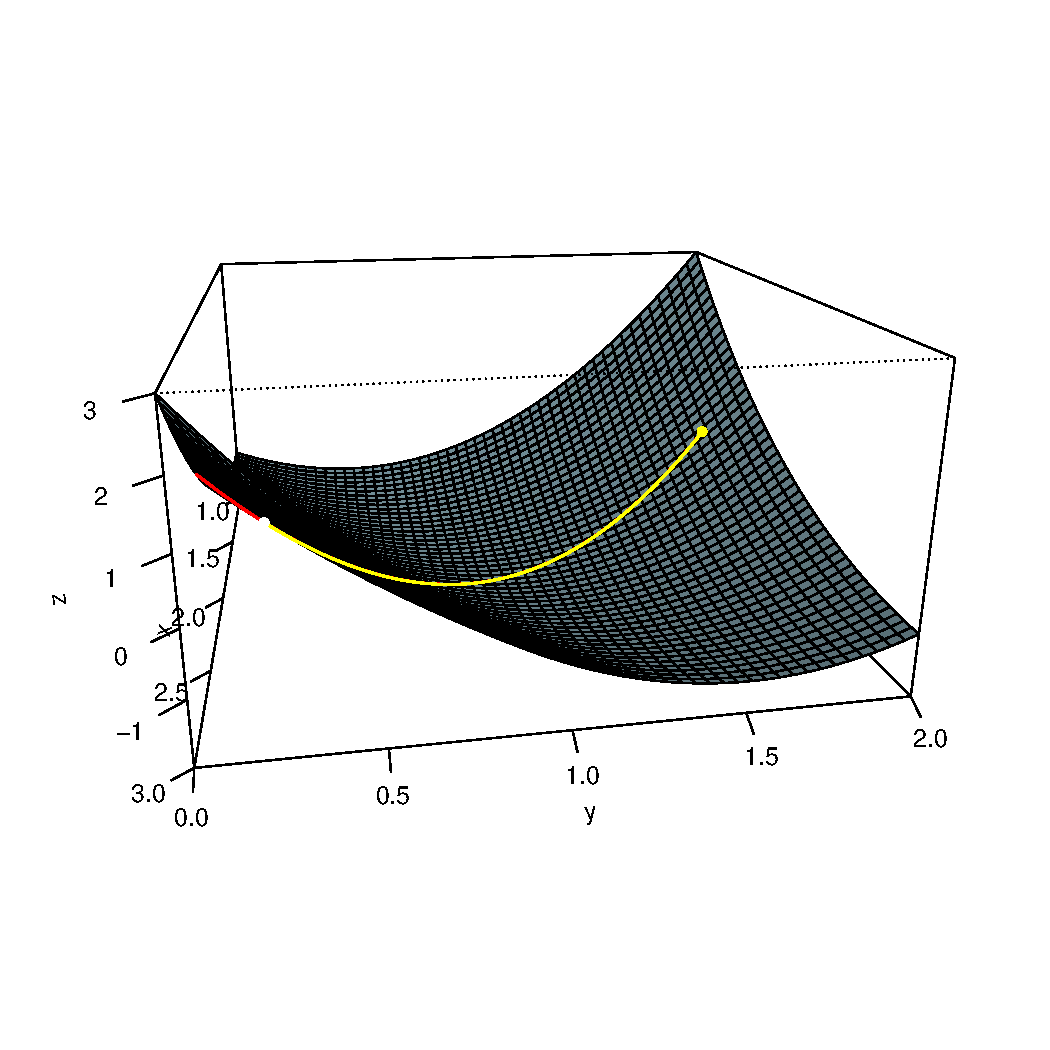
\includegraphics[width=\textwidth]{../graphs/gregory_fun/newt/newt1.pdf}
% % \captionof{figure}{\small función G-K en $x_0=(4,-4)$}
% &
% 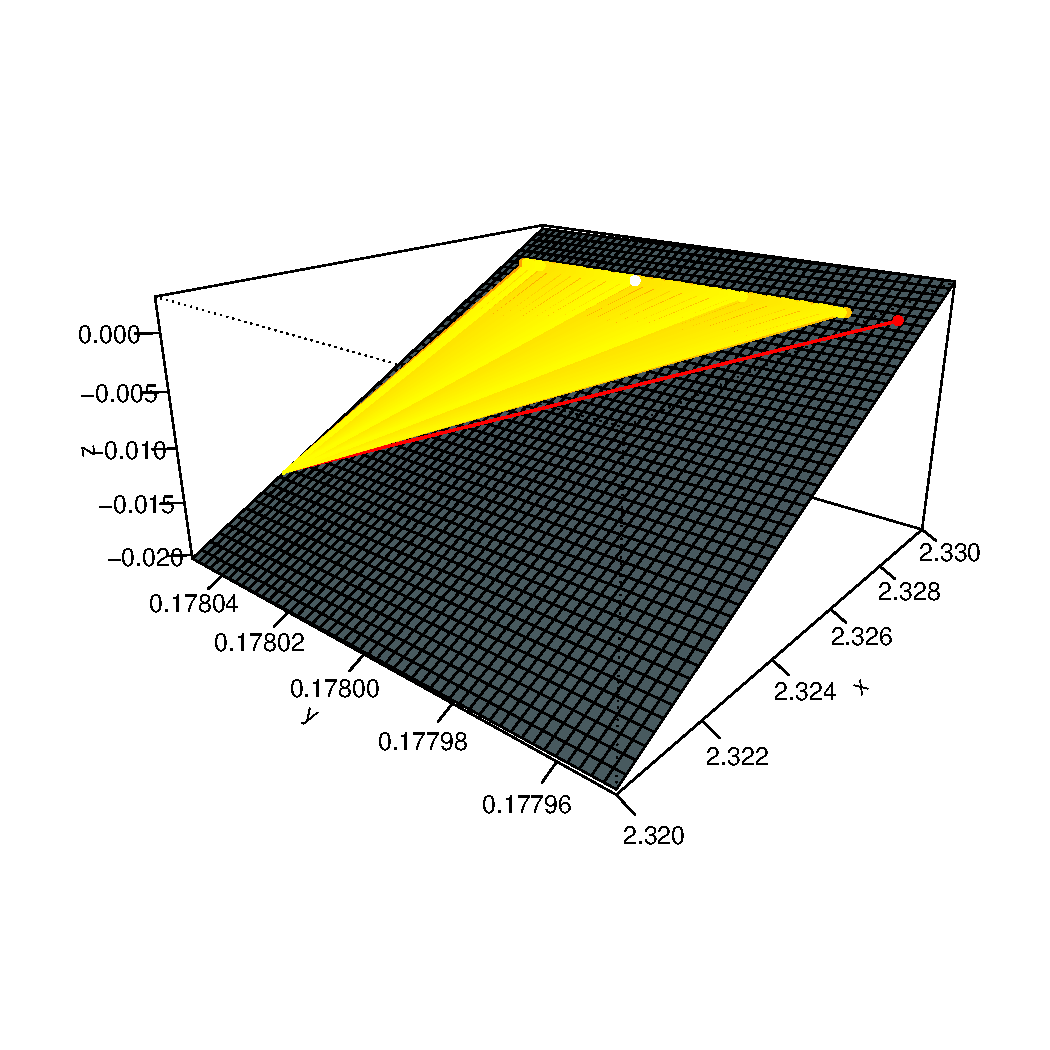
\includegraphics[width=\textwidth]{../graphs/gregory_fun/newt/newt2.pdf}
% % \captionof{figure}{\small detalles de función G-K en $x_0=(4,-4)$}
% \end{tabular}

\section{Conclusiones}
Aunque hemos probado dos algoritmos de optimización con derivadas, estos se 
comportan relativamente mal, ciclando entre puntos, entrando en fase con las
irregularidades de la función o hasta moviéndose en sentido contrario.

En parte se debe a que los algoritmos están tal y como salen en el material 
de la asignatura, por ejemplo, Newton-Raphson modificado no está protegido. 
Además, curiosamente, el simplex se comporta muy bien en general.

El motivo por el que el simplex queda como mejor del análisis es porque 
es el que más información global maneja, mientras que la mayoría de los otros
se basan en fenómenos más locales (en las funciones rugosas por ejemplo
los basados en derivadas no aciertan bien).

Por eso, una idea de algoritmo más eficiente debería combinar la capacidad de
decisión global del simplex con la capacidad local por ejemplo del steepest
descent. Para decidir entre uno y otro se hace mediante una métrica de la
"rugosidad" de la función.

\end{document}
